\documentclass{article}

\usepackage[final]{neurips_2023}
\usepackage[utf8]{inputenc} % allow utf-8 input
\usepackage[T1]{fontenc}    % use 8-bit T1 fonts
\usepackage{hyperref}       % hyperlinks
\usepackage{url}            % simple URL typesetting
\usepackage{booktabs}       % professional-quality tables
\usepackage{amsfonts}       % blackboard math symbols
\usepackage{nicefrac}       % compact symbols for 1/2, etc.
\usepackage{microtype}      % microtypography
\usepackage{xcolor}         % colors
\usepackage{float}
\usepackage{graphicx}

\title{Classification Experiments Report 2025}

\author{% 
  Team TOOTHPASTE \AND
  Aral Cimcim (k11720457)
  \And
  Sandro Müller (k52010874)
  \And 
  Linus Madlener (k12310088)
  \And 
  Kevin Eberl (k12322451)
}

\begin{document}

\maketitle

\begin{contributions}
    \textcolor{gray}{
    Aral \\
    Linus \\
    Sandro \\
    Kevin \\
    }
  
  % \textcolor{gray}{E.g.: Tara Jadidi did the entire experimental setup, including the data-split and selection of features and pre-processing. Florian Schmid trained four different classifiers for the task, and Paul Primus was responsible for evaluating the classifiers, generating figures and writing the report.}
\end{contributions}

\section{Labeling Function}
We have selected the following files with multiple sound events to assess if the labeling functions could capture the intended classes:

\textbf{677254.mp3:}

This file was annotated three times with each annotation describing it as "A musical instrument similar to a piano is playing." The length of the annotated onset and offset varies for each annotation between 0.02 - 0.65, 9.43 - 26.51, and 2.18 - 4.15 seconds. The recording consists of two people playing saxophone and piano simultaneously. The labeling functions did capture the intended classes in the recording. The free text annotations do mention "piano" but the word "saxophone" is missing. However, it is worth mentioning that the original caption for this file uses the description "piano" (for a detailed graph see \autoref{fig1}). The labeled events were clearly audible in the recording.

\begin{figure}
  \centering
  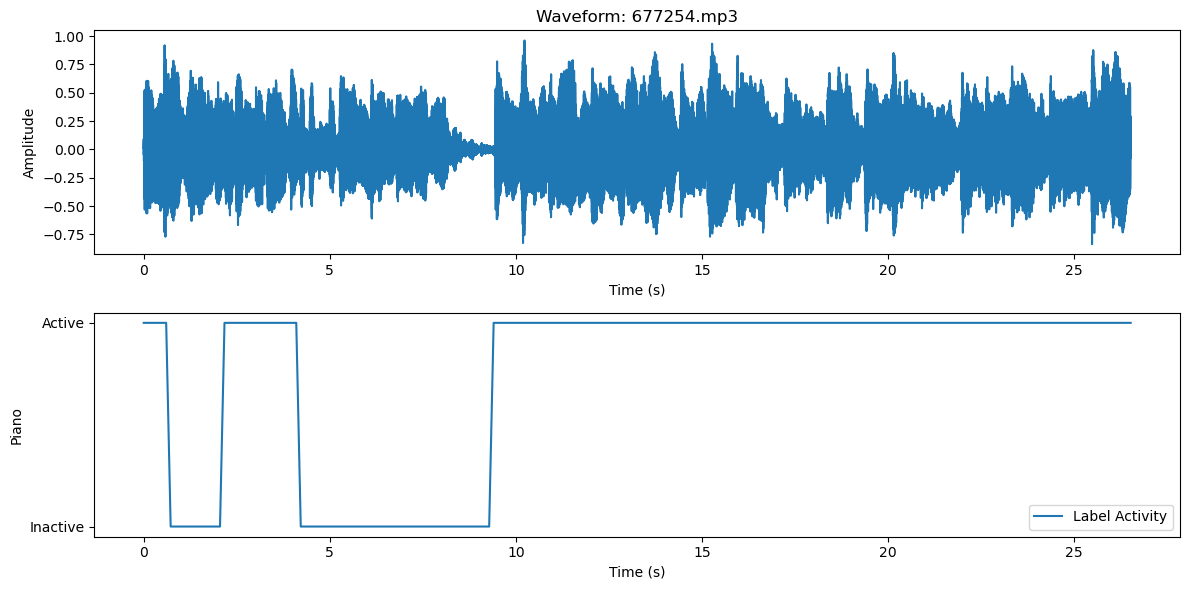
\includegraphics[width=\linewidth]{output1.png}
  \caption{Analysis of the mapped class using the labeling function.}
  \label{fig1}
\end{figure}

\textbf{231710.mp3:}

This file was annotated five times with the descriptions "rhythmic drumming", "a man is talking nearby". The beginning of the file includes a drum part for 5 seconds and then a two men begin to have a conversation. The original captions match the free-text annotations. The labeling function has correctly identified the partitions of the file as "Speech" and "Drums" (for a detailed graph \autoref{fig2}). All sound events in the file are clearly audible.

-- PARTS b) and c) are missing, I did not fully understand what to do there yet. --

\begin{figure}
  \centering
  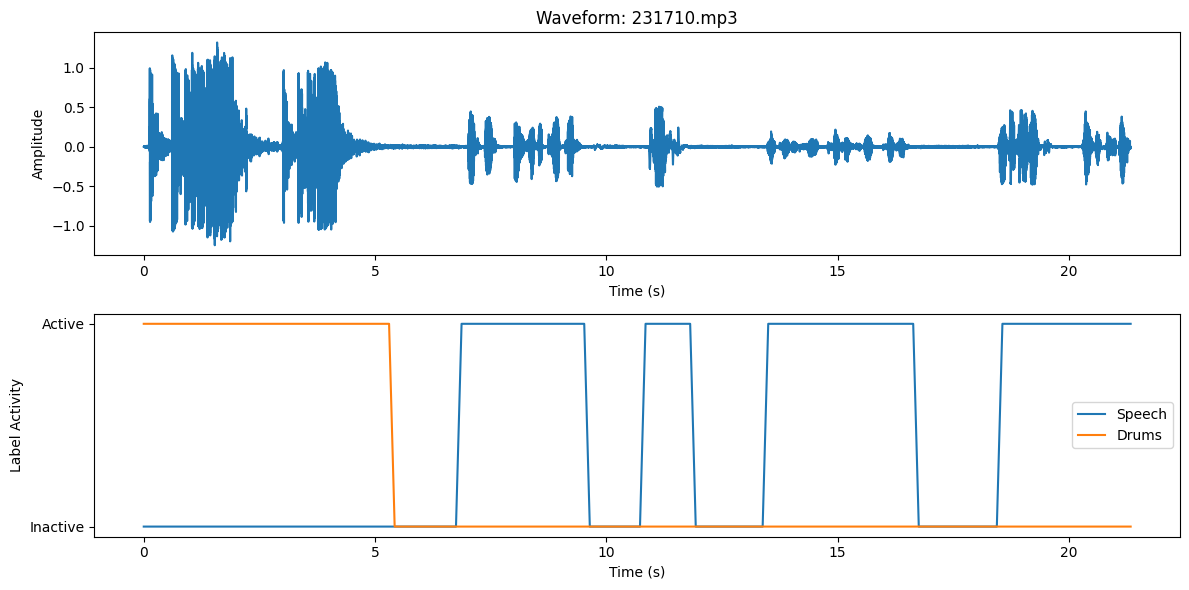
\includegraphics[width=\linewidth]{output2.png}
  \caption{Using the waveform to assess if the labels were correctly identified.}
  \label{fig2}
\end{figure}

\section{Data Split}
We have decided to use 80 \% of the data for training (so that the model has enough examples to generalize) with 10\% for validation (to reduce overfitting) and 10\% for testing (to estimate the model's unbiased performance). The training set was used for cross-validation and the validation set was used for fine-tuning the hyperparameters. The remaining 10\% was used to evaluate the model's performance.

Yes, there are potential risks for information leakage, namely, if the features in the training set are highly correlated with the labels of the test set, this could cause feature leakage. Avoiding to use features from the test set could prevent this type of leakage. 

There could also be issues with multiple recordings of the same subject such as "wind" where the model could rely heavily on these subject-specific aspects of the data. One way to address this would be to split the data in such a way that the samples containing information about the same subject are either only in the test set or the training set. 

Semantic similarity of class labels could be another issue where the annotation embeddings could have high similarity for certain classes and text embeddings. 



\section{Audio Features}


\section{Evaluation}


\section{Experiments}


\section{Analyzing Predictions}


\end{document}